\documentclass[12pt]{article}

\usepackage[bottom = 15mm]{geometry}
\usepackage[utf8]{inputenc}
\usepackage[T2A]{fontenc}
\usepackage[russian]{babel}
\usepackage{graphicx}
\usepackage{float}
\usepackage{caption}
\usepackage{amssymb, gensymb, amsmath}
\usepackage{mathrsfs}
\usepackage{array, colortbl}
\usepackage{multicol}


\textwidth = 16 cm
\textheight = 23  cm
\oddsidemargin = 0 pt
\topmargin = -1.5 cm
\parindent = 20 pt
\parskip = 0 pt
\flushbottom


\title{{\bf Задача 4.\,3.\,3 \\ Исследование разрешающей способности микроскопа методом Аббе}}
\author{Лось Денис (группа 611)}
\date{20 мая 2018}

\begin{document}

\maketitle

\paragraph*{Цель работы: } определение дифракционного предела разрешения объектива микроскопа методом Аббе, проведения исследования средствами различных способов.

\paragraph*{В работе используются: } лазер, кассета с набором сеток разного периода, линзы, щель с микрометрическим винтом, оптический стол с набором рейтеров и крепёжных винтов, экран, линейнка.

\section*{Теоритическое введение}
\par
	Всякая оптическая система, предназначенная для получения изображений, имеет конечный предел разрешения, т.е. ограниченную возможность раздельного наблюдения близко расположенных предметов. Принципиальной причиной, ограничивающей предел разрешения, является дифракция световых волн. Разрешающей способностью оптического прибора называют минимальное расстояние $l_\text{min}$ между двумя точками в пространстве предметов, которые прибор может разрешить. При визуальном наблюдении изображения в качестве критерия разрешения применяют так называемый критерий Релея.
\par
	Для иммерсионного микроскопа (объект находится в иммерсионной среде --- жидкости с показателем преломления $n$) разрешающая способность объектива при некогерентном освещении
\[
	l_\text{min} \approx \frac{0.61 \lambda}{n \sin A},
\]
где $A$ --- аппертурный угол объектива микроскопа, т.е. угол между оптической осью и лучом, направленным из центра объекта в край линзы.
\par
	Если рассматривать когерентно освещенный объект, наблюдаемый в микроскоп, то можно представить схему образования изображения в объективе микроскопа.
\begin{figure}[h!]
	\centering
	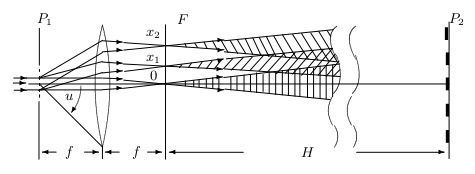
\includegraphics[width = 10cm, height = 4cm]{image2.png}
\end{figure}
\par
	Минимальное разрешаемое объективом расстояние определяется условием
\[
	l_\text{min} \approx \frac{\lambda}{\sin A} \approx \frac{\lambda}{D / 2f},
\]
где $D$ --- диаметр диафрагмы.
\par
	В нашей работе применяется двумерная решётка --- сетка. Её можно рассматривать как две скрещённые (перпендикулярные друг другу) решётки. Узкий пучок монохроматического света, пройдя через решётку с вертикальными штрихами, даёт совокупность максимумов, расположенных вдоль горизонтальной линии. Световой пучок, соотвествующий каждому максимуму, проходя через вторую решётку, распадается на новую совокупность световых пучков, дающих максимумы вдоль вертикальной линии. Главные максимумы возникают тогда, когда одновременно выполняются условия:
\[
	d \sin \theta_x = m_x \lambda \quad d \sin \theta_y = m_y \lambda
\]
где $m_x$, $m_y$ --- целые числа, характеризующие порядки дифракционных максимумов, $\theta_x$, $\theta_y$ --- направления на главные дифракционные максимумы в горизонтальной и вертикальной плоскостях соотвественно.
\section*{Экспериментальная установка}
\par
	Схема модели проекционного микроскопа приведена на рис.1. Предметом служат сетки, расположенные в кассете. Смена сеток осуществляется поворотов внешнего кольца кассеты.
\begin{figure}[h!]
	\centering
	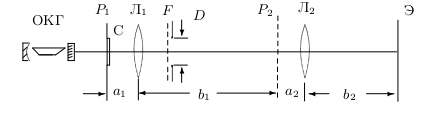
\includegraphics[width = 10cm, height = 5cm]{image1.png}
	\caption{Схема экспериментальной установки --- модель проекционного микроскопа}	
\end{figure}
\par
	Излучение лазера почти перпендикулярно падает на сетку С, установленную вблизи фокальной плоскости линзы Л1 --- объектива микроскопа.
\par
	В нашей работе период сеток рассчитывается двумя способами: в первом способе (по дифракции Фраунгофера) расстояние между дифракционными максимумами на экране измеряется при помощи линейки, а затем определяется её период, во втором способе период определяется по увеличенному (с помощью модели микроскопа) изображению сетки на экране.
\par
	С помощью откалиброванных таким образом сеток определяется разрешающая способность микроскопа. Для этого в задней фокальной плоскости F объектива устанавливается щелевая диафрагма с микрометрическим винтом и подбирается её минимальный размер, при котором ещё видно изображение сетки на экране (щель пропускает максимумы $m = 0, m \pm 1$). По размеру дифрагмы и фокусному расстоянию объектива рассчитывается аппертурный угол $u$.

\section*{Ход работы}

\subsection*{Определение периода решёток по их пространственному спектру}
\par
	Представим результаты измерения расстояния между удалёнными максимумами (горизонтальными), а также числа промежутком между ними для различных сеток.	

\begin{table}[h!]
	\centering
	\begin{tabular}{|c|c|c|c|c|}
	\hline
		$n_\text{сетки}$ & $\Delta$, мм & $k$ & $\theta_x$, рад & $d$, мкм\\
	\hline
		1 & 143 & 4 & 0.053 & 20\\
	\hline
		5 & 81 & 18 & 0.030 & 160\\
	\hline
		4 & 71 & 12 & 0.026 & 120\\
	\hline
		3 & 143 & 12 & 0.053 & 60\\
	\hline
		2 & 144 & 6 & 0.054 & 30\\		 	
	\hline
	\end{tabular}
\end{table}
\par
	Расстояние от сетки до экрана $L = 134.0 \pm 0.5$ см, длина волны лазера $\lambda = 532$ нм.
	
\paragraph*{Определение периода решёток по изображению, увеличенному с помощью модели микроскопа}
\par
	Приведём результаты измерения периодов изображений на экране.

\begin{table}[h!]
	\centering
	\begin{tabular}{|c|c|c|c|c|c|}
	\hline
		$n_\text{сетки}$ & $\delta$, мм & $b_2$, см & $a_2 + b_1$, см & $a_1$, см & $d$, мкм\\
	\hline
		1 & 0.93 & 69 & 44 & 16 & 17\\
	\hline
		2 & 1.5 & 69 & 44 & 16 & 25 \\
	\hline
		3 & 3 & 68.5 & 44.5 & 16 & 54  \\
	\hline
		4 & 6 & 68.5 & 44.5 & 16 & 109\\
	\hline
		5 & 8 & 67 & 46 & 16 & 143\\		 	
	\hline
	\end{tabular}
\end{table}
\par
	Стоит заметить, что увеличение $Г = 55$.

\section*{Определение периодов решёток по оценке разрешающей способности микроскопа}
\par
	Поместив щелевую диафрагму с микрометрическим винтом в фокальную плоскость F линзы Л1, определим для каждой решётки минимальный размер диафрагмы $D$, при котором на экране ещё видно изображение сетки (при меньших размерах щели изображение выглядит как одномерная решётка).

\begin{table}[h!]
	\centering
	\begin{tabular}{|c|c|}
	\hline
		$n_\text{сетки}$ & $D$, мм \\	
	\hline
		5 & 0.72 \\
	\hline
		4 & 1.05 \\
	\hline
		3 & 1.66 \\
	\hline
	\end{tabular}	
\end{table}

\par
	Проверим теорию Аббе, построив график зависимости $d = 	f(1 / D)$, при этому используя периоду, определённые спектральным методом.
\begin{figure}[h!]
	\centering
	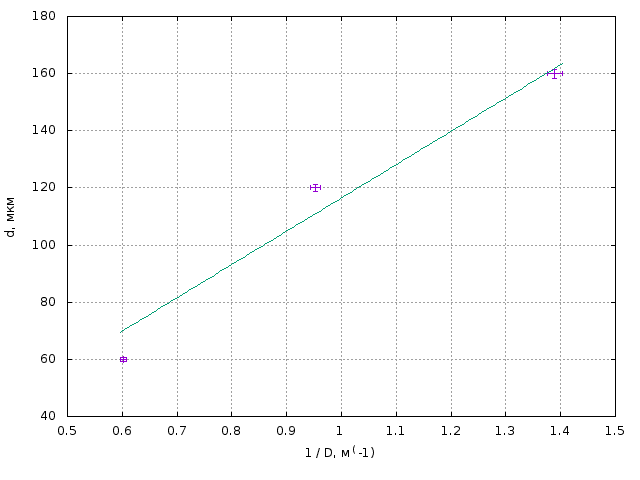
\includegraphics[width = 10cm, height = 5cm]{plot1.png}
\end{figure}
\par
	Как видно полученные значения достаточно хорошо соотвествуют линейной зависимости, а следовательно, теория Аббе имеет место быть.
\section*{Пространственная фильтрация и мультиплицирование}
\par
	Будем работать с сеткой 4. Поворачивая щель относительно оси системы, получим изображения решёток при различных ориентациях щели: для вертикального положения, для горизонтального положения и для наклонного изображения под углом $45 \degree$.
\par
	Явление мультипликации связано в основном с тем, что фильтрующая решётка пропускает дискретный спектр компонент. При этом при смене дифракцинной решётки на ту, у которой период больше, период получаемого изображения уменьшается.

\section*{Выводы}
\par
	Мы определили период диффракцинной решётки различными способами и убедились, что результаты, полученные каждым из них лежать достаточно близко. Мы также смогли экспериментально убедиться, что теория Аббе является верной. При этом нам удалось пронаблюдать такие явления как пространсвенная филтрация и мультиплицирование.
\end{document}